% Options for packages loaded elsewhere
\PassOptionsToPackage{unicode}{hyperref}
\PassOptionsToPackage{hyphens}{url}
%
\documentclass[
  11pt,
  ignorenonframetext,
  aspectratio=43]{beamer}
\usepackage{pgfpages}
\setbeamertemplate{caption}[numbered]
\setbeamertemplate{caption label separator}{: }
\setbeamercolor{caption name}{fg=normal text.fg}
\beamertemplatenavigationsymbolsempty
% Prevent slide breaks in the middle of a paragraph
\widowpenalties 1 10000
\raggedbottom
\setbeamertemplate{part page}{
  \centering
  \begin{beamercolorbox}[sep=16pt,center]{part title}
    \usebeamerfont{part title}\insertpart\par
  \end{beamercolorbox}
}
\setbeamertemplate{section page}{
  \centering
  \begin{beamercolorbox}[sep=12pt,center]{part title}
    \usebeamerfont{section title}\insertsection\par
  \end{beamercolorbox}
}
\setbeamertemplate{subsection page}{
  \centering
  \begin{beamercolorbox}[sep=8pt,center]{part title}
    \usebeamerfont{subsection title}\insertsubsection\par
  \end{beamercolorbox}
}
\AtBeginPart{
  \frame{\partpage}
}
\AtBeginSection{
  \ifbibliography
  \else
    \frame{\sectionpage}
  \fi
}
\AtBeginSubsection{
  \frame{\subsectionpage}
}
\usepackage{amsmath,amssymb}
\usepackage{lmodern}
\usepackage{iftex}
\ifPDFTeX
  \usepackage[T1]{fontenc}
  \usepackage[utf8]{inputenc}
  \usepackage{textcomp} % provide euro and other symbols
\else % if luatex or xetex
  \usepackage{unicode-math}
  \defaultfontfeatures{Scale=MatchLowercase}
  \defaultfontfeatures[\rmfamily]{Ligatures=TeX,Scale=1}
\fi
\usetheme[]{Madrid}
% Use upquote if available, for straight quotes in verbatim environments
\IfFileExists{upquote.sty}{\usepackage{upquote}}{}
\IfFileExists{microtype.sty}{% use microtype if available
  \usepackage[]{microtype}
  \UseMicrotypeSet[protrusion]{basicmath} % disable protrusion for tt fonts
}{}
\makeatletter
\@ifundefined{KOMAClassName}{% if non-KOMA class
  \IfFileExists{parskip.sty}{%
    \usepackage{parskip}
  }{% else
    \setlength{\parindent}{0pt}
    \setlength{\parskip}{6pt plus 2pt minus 1pt}}
}{% if KOMA class
  \KOMAoptions{parskip=half}}
\makeatother
\usepackage{xcolor}
\newif\ifbibliography
\usepackage{longtable,booktabs,array}
\usepackage{calc} % for calculating minipage widths
\usepackage{caption}
% Make caption package work with longtable
\makeatletter
\def\fnum@table{\tablename~\thetable}
\makeatother
\usepackage{graphicx}
\makeatletter
\def\maxwidth{\ifdim\Gin@nat@width>\linewidth\linewidth\else\Gin@nat@width\fi}
\def\maxheight{\ifdim\Gin@nat@height>\textheight\textheight\else\Gin@nat@height\fi}
\makeatother
% Scale images if necessary, so that they will not overflow the page
% margins by default, and it is still possible to overwrite the defaults
% using explicit options in \includegraphics[width, height, ...]{}
\setkeys{Gin}{width=\maxwidth,height=\maxheight,keepaspectratio}
% Set default figure placement to htbp
\makeatletter
\def\fps@figure{htbp}
\makeatother
\setlength{\emergencystretch}{3em} % prevent overfull lines
\providecommand{\tightlist}{%
  \setlength{\itemsep}{0pt}\setlength{\parskip}{0pt}}
\setcounter{secnumdepth}{-\maxdimen} % remove section numbering
\definecolor{links}{HTML}{2A1B81}
\hypersetup{colorlinks,linkcolor=,urlcolor=links}

\setbeamertemplate{items}[ball] 
\setbeamertemplate{blocks}[rounded][shadow=true] 
\setbeamertemplate{navigation symbols}{}
\setbeamertemplate{footline}{}

\setbeamersize{text margin left=1cm,text margin right=1cm} 

\usepackage{alltt}
\usepackage{multicol}
\usepackage{multirow}
\usepackage{tabulary}

% For absolute positioning of text (e.g. little footlines)
\usepackage[absolute,overlay]{textpos} 
	
% Color commands
  \definecolor{darkblue}{rgb}{0,0,.3}
  \definecolor{verylightblue}{rgb}{.9,.95,.99}
  \definecolor{lightblue}{rgb}{.5,.6,.95}
	\definecolor{green1}{rgb}{0,.5,.4}
	\definecolor{cream1}{rgb}{.97,.97,.83}
	\definecolor{deepcream}{rgb}{.2,.2,.05}
	\definecolor{emphasis}{rgb}{0,.5,.1}
	\definecolor{brightred}{rgb}{.95,.6,.6}
	\definecolor{white}{rgb}{1,1,1}	
	\definecolor{yellow}{rgb}{1,1,0}	
	\definecolor{darkgreen}{rgb}{0,0.2,0}
	\definecolor{darkorange}{rgb}{0.4,0.3,0}
	\definecolor{darkred}{rgb}{0.7,0,0}
	\definecolor{lightgray}{gray}{0.9}
	\definecolor{lightred}{rgb}{1,.5,.5}
	
	\newcommand{\drd}{\textcolor{darkred}}
	\newcommand{\rd}{\textcolor{red}}
	\newcommand{\lrd}{\textcolor{lightred}}		
	\newcommand{\bl}{\textcolor{blue}}
	\newcommand{\gr}{\textcolor{darkgreen}}
	\newcommand{\blk}{\textcolor{black}}
	\newcommand{\wt}{\textcolor{white}}
	\newcommand{\crm}{\textcolor{cream1}}
	
	\setbeamerfont{small}{size=\small}
	\setbeamerfont{smaller}{size=\footnotesize}
	\setbeamerfont{tiny}{size=\tiny}
	\setbeamerfont{teeny}{size=\scriptsize}
	
	
	\setbeamercolor{uppercol}{fg=cream1,bg=darkorange}
	\setbeamercolor{lowercol}{fg=black,bg=cream1}
  %\setbeamercolor{boxcolor}{fg=cream1,bg=green1}
	%\setbeamercolor{boxcolor1}{fg=white,bg=darkorange}
	%\setbeamercolor{boxcolor2}{fg=black,bg=cream1}
  \setbeamercolor{titlelike}{bg = darkgreen, fg = white}
  \setbeamercolor{block title}{bg = darkorange, fg = white}
	\setbeamercolor{block body}{bg = cream1, fg = black}
	  
	\newcommand{\BackH}[1]{\setbeamertemplate{background canvas}{\includegraphics[height=\paperheight]{#1}}}
	\newcommand{\BackW}[1]{\setbeamertemplate{background canvas}{\includegraphics[width=\paperwidth]{#1}}}
	\newcommand{\BackPlain}{\setbeamertemplate{background canvas}{}}
	
	\newcommand{\PlotH}[2][1]{\includegraphics[height=#1\textheight]{#2}}
	\newcommand{\PlotW}[2][1]{\includegraphics[width=#1\textwidth]{#2}}

\newcommand{\MultiPlotH}[3][1]{\includegraphics[height=#1\textheight, page=#2]{#3}}
\newcommand{\MultiPlotW}[3][1]{\includegraphics[width=#1\textwidth, page=#2]{#3}}

\setbeamercolor{itemize item}{fg = black}
\setbeamercolor{itemize subitem}{fg = black}
\setbeamercolor{enumerate item}{fg = black}
\setbeamercolor{enumerate subitem}{fg = black}


% itemization commands
%
	\newcommand{\bi}{\begin{itemize}}
	\newcommand{\ei}{\end{itemize}}
	\newcommand{\I}{\item}
	\newcommand{\ben}{\begin{enumerate}}
	\newcommand{\een}{\end{enumerate}}
	
	\newcommand{\bcol}{\begin{columns}}
	\newcommand{\col}[1][.5]{\column{#1\textwidth} }
	\newcommand{\ecol}{\end{columns}}

	\newcommand{\bc}{\begin{center}}
	\newcommand{\ec}{\end{center}}
	
	\newcommand{\beq}{\begin{equation*}}
	\newcommand{\eeq}{\end{equation*}}
	
	\newcommand{\beqrray}{\begin{eqnarray*}}
	\newcommand{\eeqrray}{\end{eqnarray*}}
	
	\newcommand{\bbb}[1]{\begin{beamerboxesrounded}[upper=uppercol,lower=lowercol,shadow=false]{#1}}			
	\newcommand{\ebb}{\end{beamerboxesrounded}}

	\newcommand{\nd}{\vspace{.1in}}
	\newcommand{\nup}{\vspace{-.1in}}
	\newcommand{\nl}{\hspace{-.1in}}
	\newcommand{\nr}{\hspace{+.1in}}
	
% Creates little textblocks!?
	\newcommand\FrameText[1]{
	  \begin{textblock*}{\paperwidth}(0pt,1pt)
	    \raggedright #1
	  \end{textblock*}}
	

\ifLuaTeX
  \usepackage{selnolig}  % disable illegal ligatures
\fi
\IfFileExists{bookmark.sty}{\usepackage{bookmark}}{\usepackage{hyperref}}
\IfFileExists{xurl.sty}{\usepackage{xurl}}{} % add URL line breaks if available
\urlstyle{same} % disable monospaced font for URLs
\hypersetup{
  pdftitle={Can Selective Predation Slow the Spread of CWD?},
  pdfauthor={Dr.~Elie Gurarie \textbar{} SUNY-ESF},
  hidelinks,
  pdfcreator={LaTeX via pandoc}}

\title{Can Selective Predation Slow the Spread of CWD?}
\subtitle{Modeling disease, predation, dispersal, and population
dynamics in Wisconsin}
\author{Dr.~Elie Gurarie \textbar{} SUNY-ESF}
\date{November 29, 2022}

\begin{document}
\frame{\titlepage}

\begin{frame}{The setting: \textbf{Wisconsin}}
\protect\hypertarget{the-setting-wisconsin}{}
\PlotW{../images/Wisconsin_in_United_States.png}
\end{frame}

\begin{frame}{The setting: \textbf{Wisconsin}}
\protect\hypertarget{the-setting-wisconsin-1}{}
\bc \PlotW[.45]{../images/WisconsinVegetation}
\PlotW[.45]{../images/TensionZone} \ec

\begin{itemize}
\tightlist
\item
  \textbf{Southwest:} Mainly agricultural / ex-prairie and oak savanna.
\item
  \textbf{Northeast:} Conifer-hardwood forest / bogs / also agriculture
\end{itemize}
\end{frame}

\begin{frame}{The setting: \textbf{Wisconsin}}
\protect\hypertarget{the-setting-wisconsin-2}{}
\bc  \PlotW[.7]{../images/Treaty1837} \ec Wildlife management and
fishing rights largely retained by Ojibwe tribes in the North.
\end{frame}

\begin{frame}{Three characters}
\protect\hypertarget{three-characters}{}
\Large

\begin{enumerate}
\tightlist
\item
  White-tailed deer
\item
  Chronic wasting disease
\item
  Wolves
\end{enumerate}
\end{frame}

\begin{frame}{White-tailed deer in Wisconsin}
\protect\hypertarget{white-tailed-deer-in-wisconsin}{}
\bcol

\col[.6]

\bbb{\emph{Odoiceulus virginiacus}}

\small

\begin{itemize}
\tightlist
\item
  (over)-abundant: 1.9-2.1 million ind.
\item
  major ecological impacts
\item
  \(\approx\) 350,000 hunted annually (and falling)
\item
  \$1.4 billion dollars / year to economy
\item
  a big chunk of which funds research / mitigation of those ecological
  impacts
\end{itemize}

\ebb

\col[.4]
\PlotW{../images/deer}
\bc\scriptsize \bl{Todd Hubler - \emph{The Isthmus}}\ec
\ecol
\end{frame}

\begin{frame}{Chronic Wasting Disease}
\protect\hypertarget{chronic-wasting-disease}{}
\bcol

\col[.6]

\small

\bbb{Transmissible spongiform encephalopathy}

\begin{itemize}
\tightlist
\item
  Turns brains into sponges
\item
  Invariably fatal
\item
  Caused by \textbf{prion}

  \begin{itemize}
  \tightlist
  \item
    misfolded protein found in nervous system
  \end{itemize}
\item
  Only affects cervids

  \begin{itemize}
  \tightlist
  \item
    only TSE in \emph{wildlife}
  \end{itemize}
\item
  Major focus of concern / research among agencies
\end{itemize}

\ebb

\col[.4]

\PlotW{../images/misfold}
\PlotW{../images/bse_sponge}

\ecol
\end{frame}

\begin{frame}{Chronic Wasting Disease}
\protect\hypertarget{chronic-wasting-disease-1}{}
\bcol

\col[.5]

\small

\bbb{Clinical Signs}

``Zombie Disease''

\begin{itemize}
\tightlist
\item
  Emaciation
\item
  Lack of coordination
\item
  Drooping head/ears
\item
  Excessive drooling
\item
  Excessive drinking
\item
  Excessive urination
\end{itemize}

\ebb

\col[.5]

\PlotW{../images/sickdeer}
\ecol

\textbf{Incubation:} (asymptomatic) period lasts on average 18 months

\textbf{Transmission:} urine, feces, blood. Direct contact. Long-term
environmental persistence (even uptake by plants).
\end{frame}

\begin{frame}{Chronic Wasting Disease - life cycle}
\protect\hypertarget{chronic-wasting-disease---life-cycle}{}
\PlotW{../images/CWD_lifecycle.jpg}
\end{frame}

\begin{frame}{Chronic Wasting Disease}
\protect\hypertarget{chronic-wasting-disease-2}{}
\bcol

\col[.4]

\footnotesize

\bbb{Global Expansion}

\begin{itemize}
\tightlist
\item
  1967 - First detected (mule deer) in research facility Colorado.
\item
  1981 - First wild animal (elk) detected in Colorado
\item
  2002 - Found in wild WTD in Wisconsin
\item
  2011 - Found in wild WTD in Maryland
\item
  2017 - Appeared in 3 reindeer in Norway (!) - entire 2000 animal herd
  summarily executed
\end{itemize}

\ebb

\col[.6]

\PlotW{../images/CWD_NorthAmerica}

\ecol
\end{frame}

\begin{frame}{Chronic Wasting Disease: In Wisconsin}
\protect\hypertarget{chronic-wasting-disease-in-wisconsin}{}
Concentrated in southern counties, up to 25\% prevalance.

\bc \PlotW[.6]{../images/CWDprevalence} \ec

\textbf{\emph{Good data:}} In affected counties, all hunted carcasses
need to be tested. In non-affected counties, a sample of carcasses is
tested.
\end{frame}

\begin{frame}{Wolves in Wisconsin}
\protect\hypertarget{wolves-in-wisconsin}{}
\small

Extirpated early 1900's. Re-colonized from Minnesota post-ESA.

\bcol

\col

\PlotW[.9]{../images/WolfMap2019}

\col

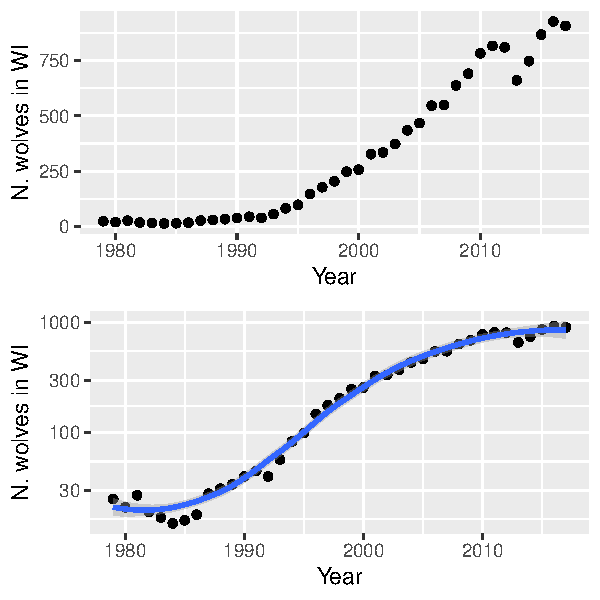
\includegraphics{deer_wolf_CWD_files/figure-beamer/WolfNums-1.pdf}

\ecol

Currently, approx. 1000 ind. mainly in North. Expansion slowing.
\textbf{\emph{Good Data.}}
\end{frame}

\begin{frame}{The question}
\protect\hypertarget{the-question}{}
\small

Wolves selectively predate on old, young, weak or \textbf{infirm(?)}
individuals \ldots{} though there is no direct evidence w.r.t. CWD (or -
actually - other diseases).

Given that CWD is concentrated in the SW - and expanding - and wolves
are concentrated in NE - and maybe still expanding? - What happens when
they meet?

Specifically, how do wolf presence and selective predation influence:

\begin{itemize}
\tightlist
\item
  \textbf{CWD prevalence}
\item
  \textbf{CWD spread}
\item
  \textbf{Deer abundance}
\end{itemize}
\end{frame}

\begin{frame}{Approaches to look at this question}
\protect\hypertarget{approaches-to-look-at-this-question}{}
Lots of \textbf{\emph{Mathematical Modeling!!}} Mainly, continuous-time,
non-spatial SEIR-type ODE's.

\bcol
\col
\PlotW{../images/WildTitle}
\PlotW{../images/WildEquations}

Very influential, but no data (and no spatial structure)

\col
\bc
\PlotW{../images/TannerTitle}
\PlotW[0.7]{../images/TannerEquations}
\ec

Lots of compartments - and some data (but no spatial structure)

\ecol
\end{frame}

\begin{frame}{Modeling goals}
\protect\hypertarget{modeling-goals}{}
\begin{itemize}
\item
  Capturing dynamics of:

  \begin{itemize}
  \tightlist
  \item
    \textbf{disease},
  \item
    \textbf{predation},
  \item
    \textbf{population}
  \item
    \textbf{dispersal}
  \end{itemize}
\item
  Biologically meaningful parameters

  \begin{itemize}
  \tightlist
  \item
    independently estimated / estimable?
  \end{itemize}
\item
  Provide spatially and temporally explicit predictions
\item
  Balances realism with tractability
\end{itemize}
\end{frame}

\begin{frame}{Basic model structure:}
\protect\hypertarget{basic-model-structure}{}
\begin{block}{Discrete time / discrete space}
\protect\hypertarget{discrete-time-discrete-space}{}
\begin{itemize}
\item
  \textbf{Annual} - matches data collection and deer biology (birth /
  seasonal mortality / dispersal?)
\item
  \textbf{County-level metapopulation} - matches data reporting and
  collection
\end{itemize}
\end{block}

\begin{block}{Two classes: Susceptible and Infected}
\protect\hypertarget{two-classes-susceptible-and-infected}{}
\small

\begin{align}
S_{i,t+1} &= S_{i,t} - \rd{infected} & + \bl{recruited}& - \rd{died} + \bl{immigrated} - \rd{emigrated} \nonumber\\
I_{i, t+1} &= I_{i,t} + \bl{infected} & &  -\rd{died} + \bl{immigrated} - \rd{emigrated} \nonumber
\end{align}
\end{block}
\end{frame}

\begin{frame}{Complete model}
\protect\hypertarget{complete-model}{}
\bc

\scriptsize

\begin{longtable}[]{@{}
  >{\raggedright\arraybackslash}p{(\columnwidth - 4\tabcolsep) * \real{0.2308}}
  >{\centering\arraybackslash}p{(\columnwidth - 4\tabcolsep) * \real{0.3846}}
  >{\centering\arraybackslash}p{(\columnwidth - 4\tabcolsep) * \real{0.3846}}@{}}
\toprule()
\begin{minipage}[b]{\linewidth}\raggedright
\end{minipage} & \begin{minipage}[b]{\linewidth}\centering
Susceptible \((S_{i,t+1})\)
\end{minipage} & \begin{minipage}[b]{\linewidth}\centering
Infected \((I_{i,t+1})\)
\end{minipage} \\
\midrule()
\endhead
disease & \(- \gamma {S_{i,t} I_{i,t} \over area}\) &
\(\gamma{ S_{i,t} I_{i,t} \over area}\) \\
predation &
\(-\left({S_{i,t} \over S_{i,t}+I_{i,t}}\right) \left({1 \over 1 + \alpha}\right) W_{max}\)
&
\(-\left({I_{i,t} \over S_{i,t}+I_{i,t}}\right) \left({\alpha \over 1 + \alpha}\right) W_{max}\) \\
other mortality & \(- \mu_s S_{i,t}\) & \(- \mu_I I_{i,t}\) \\
recruitment & \(\rho S_{i,t}(1 - S_{i,t}/K_i)\) & \\
immigration & \(\sum_{j} M_{S,ij}\) & \(\sum_{j} M_{I,ij}\) \\
emigration & \(-\sum_{j} E_{s,ji}\) & \(-\sum_{j} E_{i,ji}\) \\
\bottomrule()
\end{longtable}

\PlotW[.7]{../images/gif/crudity_1}

\ec
\end{frame}

\begin{frame}{Data}
\protect\hypertarget{data}{}
\begin{block}{\textbf{Deer Abundance}}
\protect\hypertarget{deer-abundance}{}
Wisconsin DNR winter population survey:
\url{https://dnr.wi.gov/topic/hunt/maps.html} \bc
\PlotW[.45]{../images/overwinter.pdf}
\PlotW[.45]{../images/winterpoppertotal.pdf} \ec Fall population
estimates - total harvest, by county.

\nd Working assumption: Carrying Capacity \(K_i = 2 N_i\).
\end{block}
\end{frame}

\begin{frame}{Data}
\protect\hypertarget{data-1}{}
\begin{block}{\textbf{CWD prevalence}}
\protect\hypertarget{cwd-prevalence}{}
Wisconsin DNR CWD monitoring efforts (by county) \nd

\bc
\PlotW[.7]{../images/CWDprevalence}
\ec

\small \url{https://dnr.wi.gov/wmcwd/Summary/YearCounty/2019}
\end{block}
\end{frame}

\begin{frame}{Data}
\protect\hypertarget{data-2}{}
\begin{block}{\textbf{Wolves}}
\protect\hypertarget{wolves}{}
Latest estimate from DNR: 950 ind.

\bc \PlotH[.5]{../images/WolfMap2019.png} ,,,
\PlotH[.5]{../images/WolfMapElie.png} \ec

County data not readily available \ldots{} so I allocated 1000 wolves
across the counties north of this line.
\end{block}
\end{frame}

\begin{frame}{Model}
\protect\hypertarget{model}{}
Interactive model facilitates exploring parameters and visualizing
results.

\bc

(enjoy demo) \ec
\end{frame}

\begin{frame}[fragile]{A Result: Selective Predation Decreases CWD
Prevalence!}
\protect\hypertarget{a-result-selective-predation-decreases-cwd-prevalence}{}
\bc
\PlotW[.9]{../images/SimResults1.png}
\ec

\small

In ALL parameterizations, wolves depress CWD. Note - dispersal scale (10
and 80 km) AND shape both important.

\footnotesize \texttt{rho\ =\ 0.5,\ gamma\ =\ .02,\ mu\_S\ =\ 0.06,\ mu\_I\ =\ 0.06,\ W\_max\ =\ 60,\ lambda\ =\ 10\ or\ 80}
\end{frame}

\begin{frame}{Next steps}
\protect\hypertarget{next-steps}{}
\footnotesize

\begin{block}{Model structure}
\protect\hypertarget{model-structure}{}
\begin{itemize}
\tightlist
\item
  Add \textbf{Male / Female} sex classes!
\item
  Separate \textbf{Infected / Asymptomatic} from \textbf{Infected /
  Symptomatic}
\item
  Assess assumptions: Density dependence? \textbar{} Disease
  transmission? \pause
\end{itemize}
\end{block}

\begin{block}{Data}
\protect\hypertarget{data-3}{}
\begin{itemize}
\tightlist
\item
  Obtain better \textbf{wolf distribution} and \textbf{predation} data
\item
  Use \textbf{Harvest} for mortality!
\item
  Use \textbf{GPS data} for dispersal portion
\item
  Fit to historical data!?

  \begin{itemize}
  \tightlist
  \item
    Infer \(\gamma\) by matching to observed CWD spread? \pause
  \end{itemize}
\end{itemize}
\end{block}

\begin{block}{Larger strategy}
\protect\hypertarget{larger-strategy}{}
\begin{itemize}
\tightlist
\item
  Thoroughly analyze / explore parameter space
\item
  Find PhD student to do the work!?
\item
  Get funding!
\end{itemize}
\end{block}
\end{frame}

\begin{frame}{}
\protect\hypertarget{section}{}
\bc
\Huge

Thanks! \ec
\end{frame}

\end{document}
